\documentclass[12pt]{beamer}
\usepackage[english]{babel}
\usepackage[utf8]{inputenc}
\usepackage[T1]{fontenc}
\usepackage{lmodern}
\usepackage{minted}
\usepackage{graphicx}

\makeatletter

\setbeamersize{text margin left=1em,text margin right=1em}

\setbeamerfont{title}{series=\bfseries,size=\LARGE}
\setbeamerfont{subtitle}{series=\bfseries,size=\Large}
\setbeamerfont{frametitle}{series=\bfseries,size=\small}
\setbeamerfont{block title}{series=\bfseries,size=\normalsize}
\setbeamerfont{footline}{size=\normalsize}

\usebeamercolor{structure}
\setbeamercolor{normal text}{fg=structure.fg}

\addtobeamertemplate{frametitle}{}{\vspace*{-1ex}\rule{\textwidth}{1pt}}

\setbeamertemplate{itemize items}[circle]

\setbeamertemplate{navigation symbols}{}

\setbeamertemplate{footline}{
   \centering
   \begin{minipage}{\dimexpr\paperwidth-\beamer@leftmargin-\beamer@rightmargin\relax}
   \centering
   \rule{\linewidth}{1pt}\vskip2pt
   \usebeamerfont{footline}
   \usebeamercolor{footline}
   \hfill\insertframenumber/\inserttotalframenumber
   \hfill
   \llap{\insertframenavigationsymbol\insertbackfindforwardnavigationsymbol}\par
   \end{minipage}\vskip2pt
}

\makeatother

\newcommand{\mycomment}[1]{}

\graphicspath{ {./img/} }

\title{Tape library automation}
\author{Arena M., Corriera F., Orlando T.}
\institute{Università degli studi di Messina}
\date{05/07/2023}

\begin{document}

\begin{frame}
\maketitle
\end{frame}

\begin{frame}
\frametitle{Summary}
\begin{itemize}
\item General idea
\item Functional Requirements
\item Tools
\item Model and joints
\item Scene
\item Finite State Machine
\end{itemize}
\end{frame}

\begin{frame}
\frametitle{General Idea}
\framesubtitle{}
A tape library is a type of computer storage device that provides high-capacity data storage and retrieval using magnetic tape cartridges. It is designed to efficiently store and manage a large number of tape cartridges in an automated manner.

Two main components:
\begin{itemize}
    \item \textbf{Tape drives:} responsible for reading from and writing to the magnetic tape cartridges
    \item \textbf{Robotic mechanisms:} typically robotic arms, are used to handle and transport the tape cartridges within the library
\end{itemize}
\end{frame}

\begin{frame}
\frametitle{}
\framesubtitle{}
\begin{figure}
    \centering
    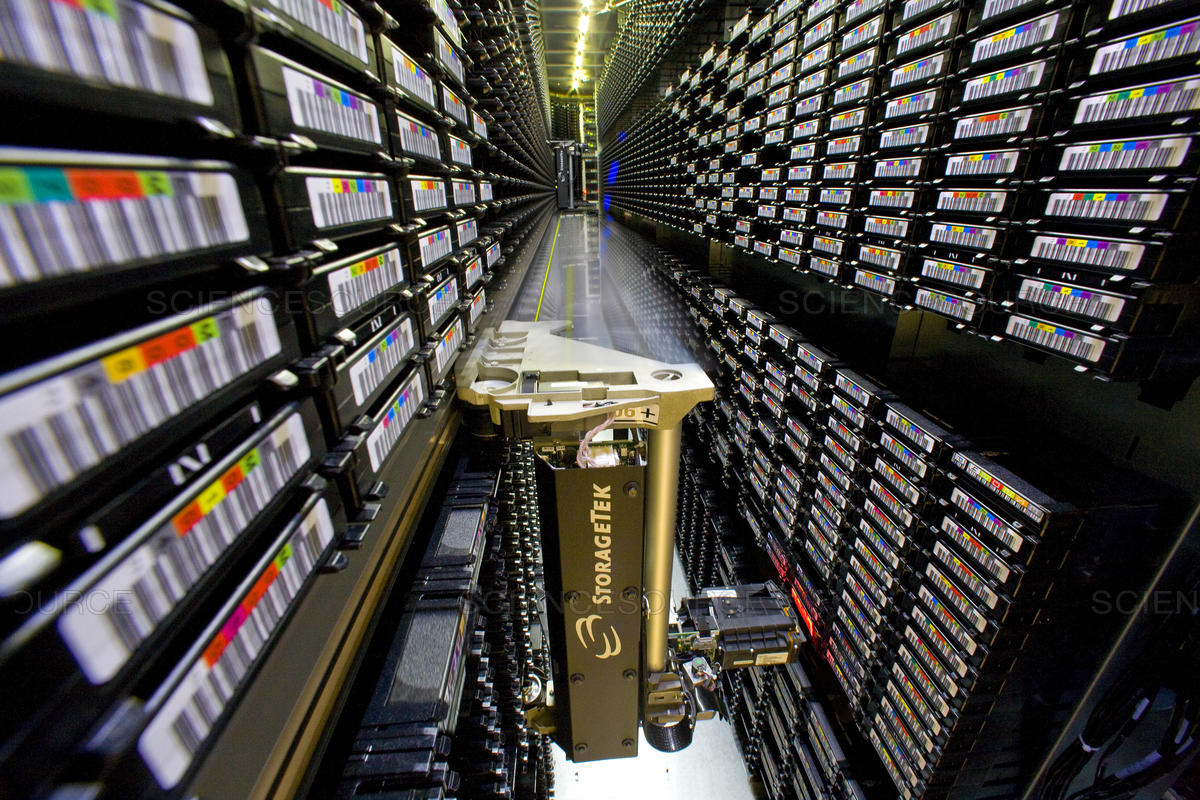
\includegraphics[trim={0 0 0 0}, clip, scale=.26]{img/storagetek_robot.jpg}
    \label{fig:tape_library}
\end{figure}
\end{frame}

\begin{frame}
\frametitle{General Idea}
\framesubtitle{The robotic arm}
The robotic arms enable the library to perform various automated tasks, but we will focus on:
\begin{itemize}
    \item Loading and unloading tape cartridges
    \item Moving the cartridges
    \item Presenting them to the tape drives for data access
\end{itemize}
\end{frame}

\begin{frame}
\frametitle{Functional Requirements}
\framesubtitle{}
\begin{itemize}
    \item The robotic arm must be able to reach any slot in the library
    \item The robotic arm must be able to take any cartridge from their slots
    \item The robotic arm must be able to move any cartridge from its slot to the drive and vice-versa
    \item The robotic arm must be able to load and unload the cartridge to and from the drive
\end{itemize}
\end{frame}

\begin{frame}
\frametitle{Tools}
\framesubtitle{}
\begin{itemize}
    \item CoppeliaSim Edu, Version 4.5.1 (rev. 5)
    \item Lua programming language (version 5.2)
    \item Autodesk Revit 2023
\end{itemize}
\end{frame}

\begin{frame}
\frametitle{Model and joints}
\framesubtitle{}
The robot is a cartesian manipulator equipped with a series of three mutually orthogonal prismatic joints.

Starting from the manipulator base, the joints are configured as follows:
\begin{enumerate}
    \item \textbf{X joint:} to align the gripper to the cartridge slot
    \item \textbf{Z joint:} to align the gripper to the shelf
    \item \textbf{Y joint:} to perform the grip
\end{enumerate}
\end{frame}

\begin{frame}
\frametitle{Model and joints}
\framesubtitle{}
\begin{figure}
    \centering
    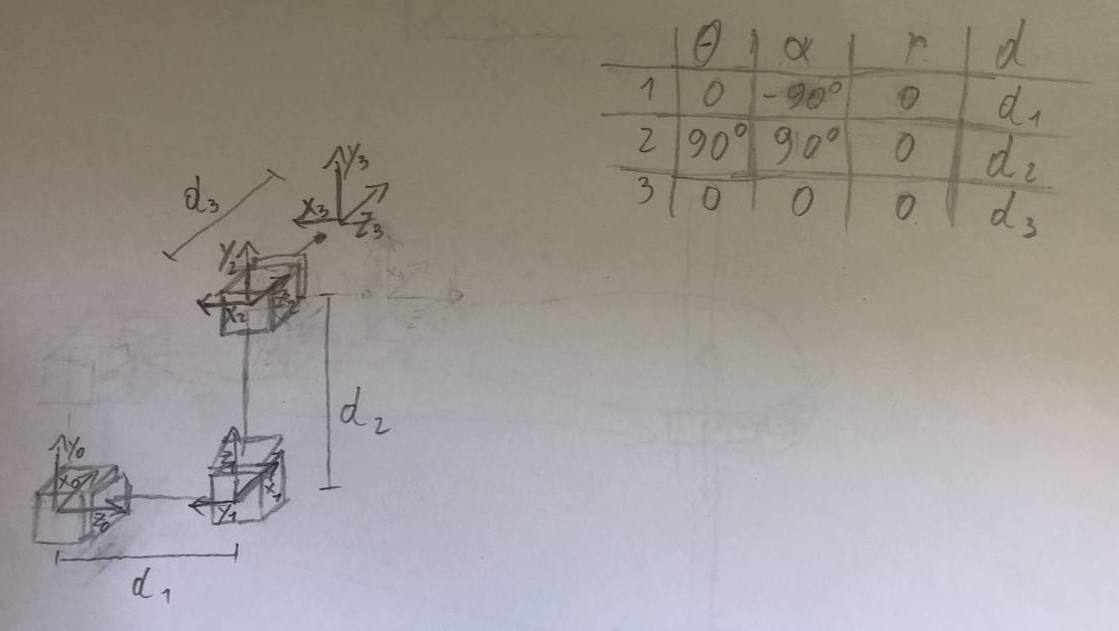
\includegraphics[height=.71\textheight, trim={0 0 0 0}, clip]{img/photo_2023-07-02_11-51-53.jpg}
    \caption{DH model and table}
    \label{fig:DH}
\end{figure}
\end{frame}

\begin{frame}
\frametitle{Model and joints}
\framesubtitle{}
The workspace is a cuboid with the following size:
\begin{itemize}
    \item X = 2.64 m
    \item Z = 1.05 m
    \item Y = 0.15 m
\end{itemize}
\end{frame}

\begin{frame}
\frametitle{Model and joints}
\framesubtitle{}
\begin{itemize}
\item The adopted end effector is the Baxter gripper, available in the CoppeliaSim model library.
\item The end effector is equipped with a laser sensor detecting the presence of the object that has to be picked up.
\item The cartridge model has been designed directly using CoppeliaSim.
\item The tape drive and the tape rack have been designed using Autodesk Revit.
\end{itemize}
\end{frame}

\begin{frame}
\frametitle{Scene}
\framesubtitle{}
\begin{figure}
    \centering
    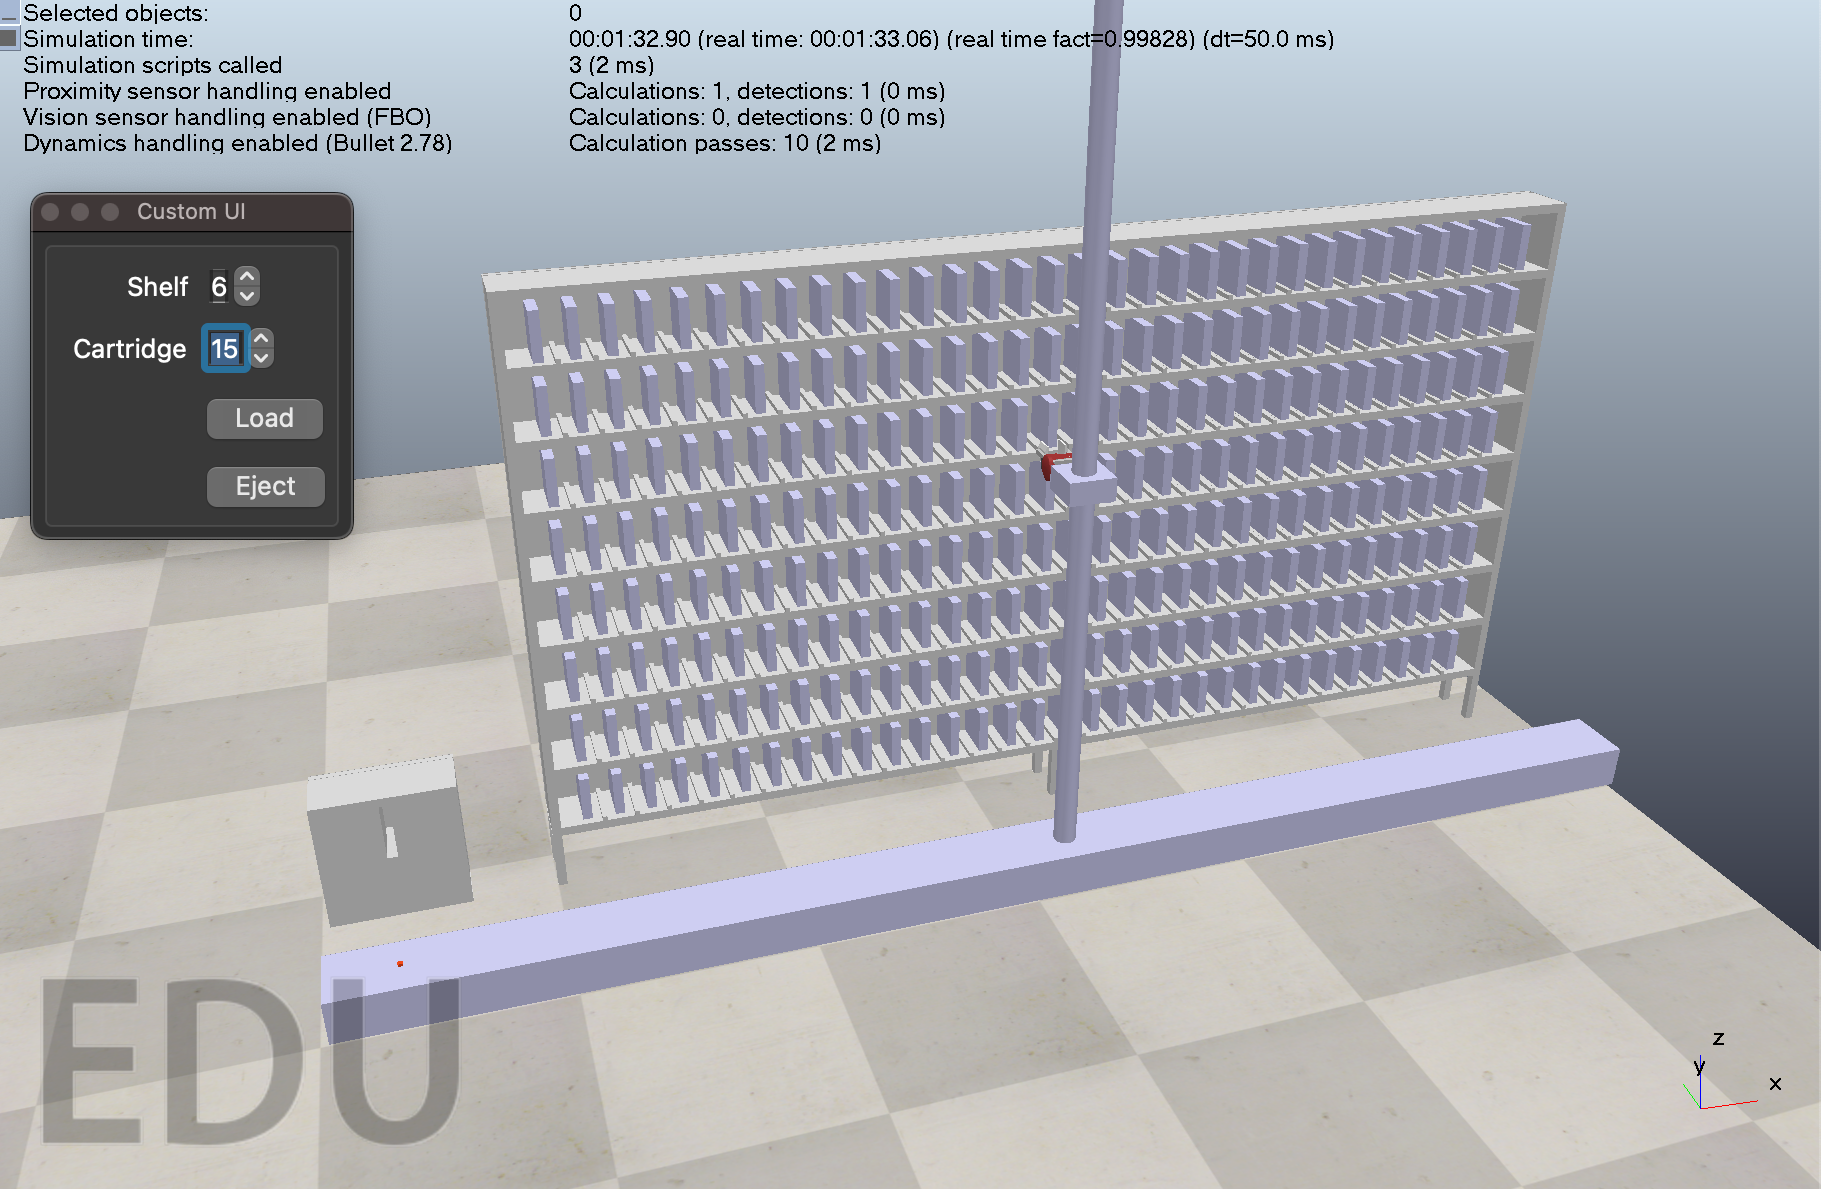
\includegraphics[height=.8\textheight, trim={0 0 0 0}, clip]{img/scene.png}
    \label{fig:coppelia_scene}
\end{figure}
\end{frame}

\begin{frame}
\frametitle{Scene}
\framesubtitle{Custom models}
\begin{figure}
    \centering
    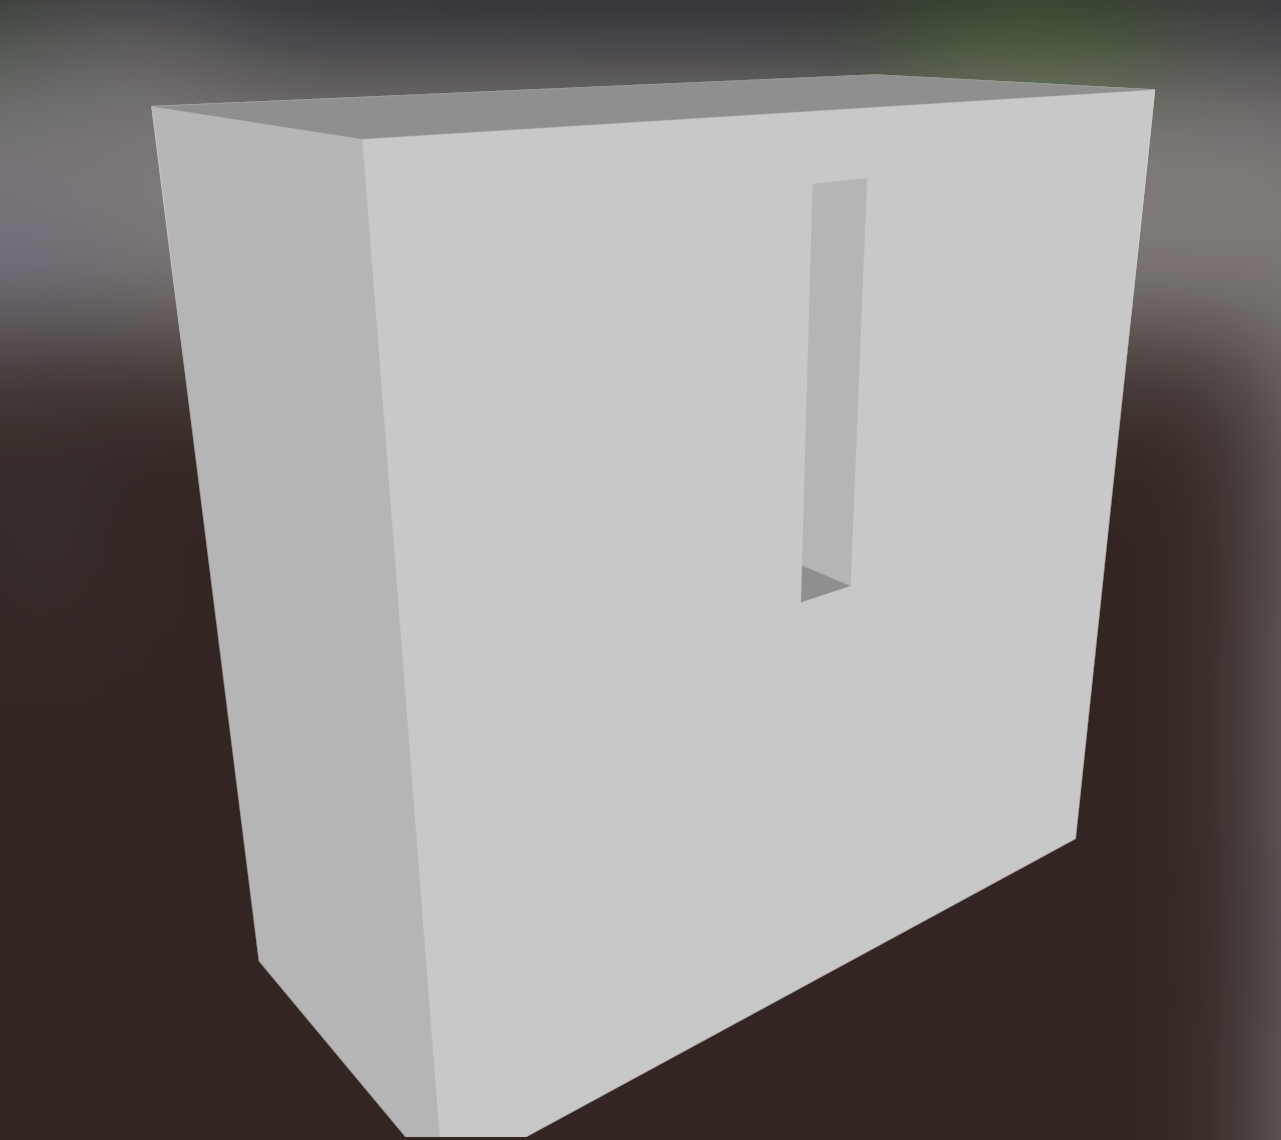
\includegraphics[width=.4\textwidth, trim={0 0 0 0}, clip]{img/drive.png}
    \caption{Drive 3d model (13.5 cm × 30 cm × 30 cm)}
    \label{fig:model_drive}
\end{figure}
\end{frame}

\begin{frame}
\frametitle{Scene}
\framesubtitle{Custom models}
\begin{figure}
    \centering
    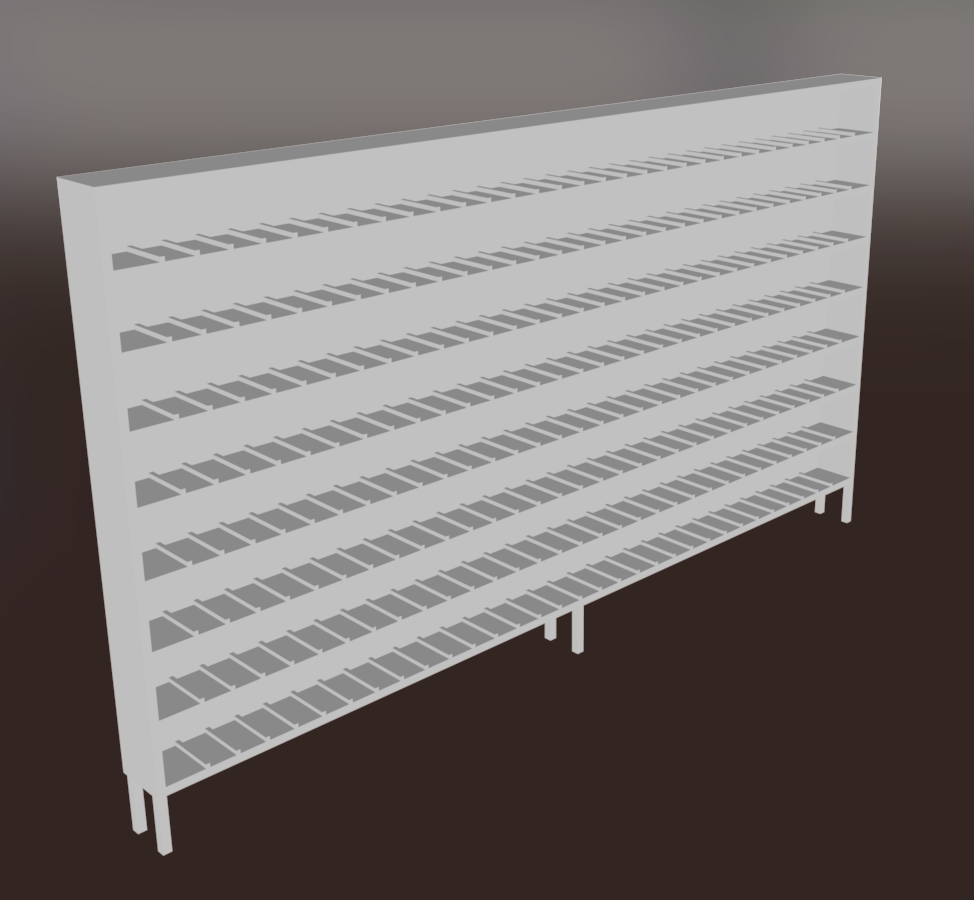
\includegraphics[width=.5\textwidth, trim={0 0 0 0}, clip]{img/rack.png}
    \caption{Rack 3d model (2.38 m × 0.135 m × 1.35 m)}
    \label{fig:model_rack}
\end{figure}
\end{frame}

\begin{frame}
\frametitle{Scene}
\framesubtitle{Custom models}
\begin{figure}
    \centering
    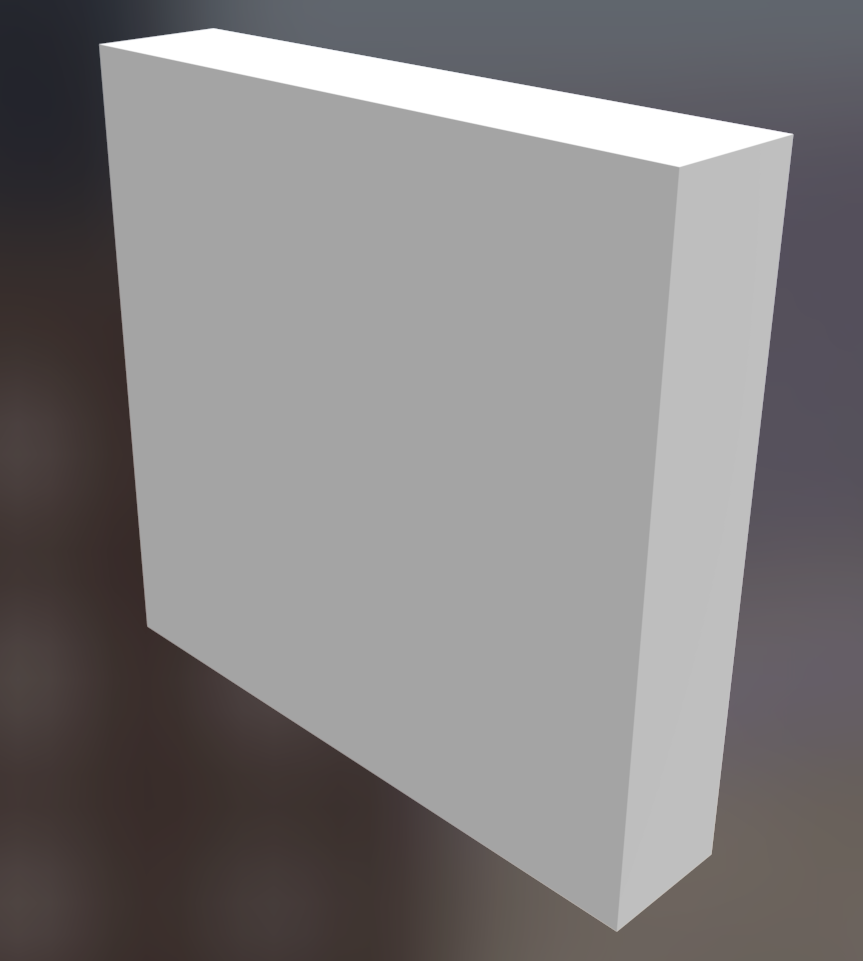
\includegraphics[width=.4\textwidth, trim={0 0 0 0}, clip]{img/cartridge.png}
    \caption{Cartridge 3d model (102.0 mm × 105.4 mm × 21.5 mm)}
    \label{fig:model_cartridge}
\end{figure}
\end{frame}

\begin{frame}
\frametitle{Scene}
\framesubtitle{Custom models}
\begin{figure}
    \centering
    
\includegraphics[width=.65\textwidth, trim={0 0 0 0}, clip]{img/manipulator.png}
    \caption{Manipulator robot}
    \label{fig:coppelia_robot}
\end{figure}
\end{frame}

\begin{frame}
\frametitle{Scene}
\framesubtitle{}
\begin{figure}
    \centering
    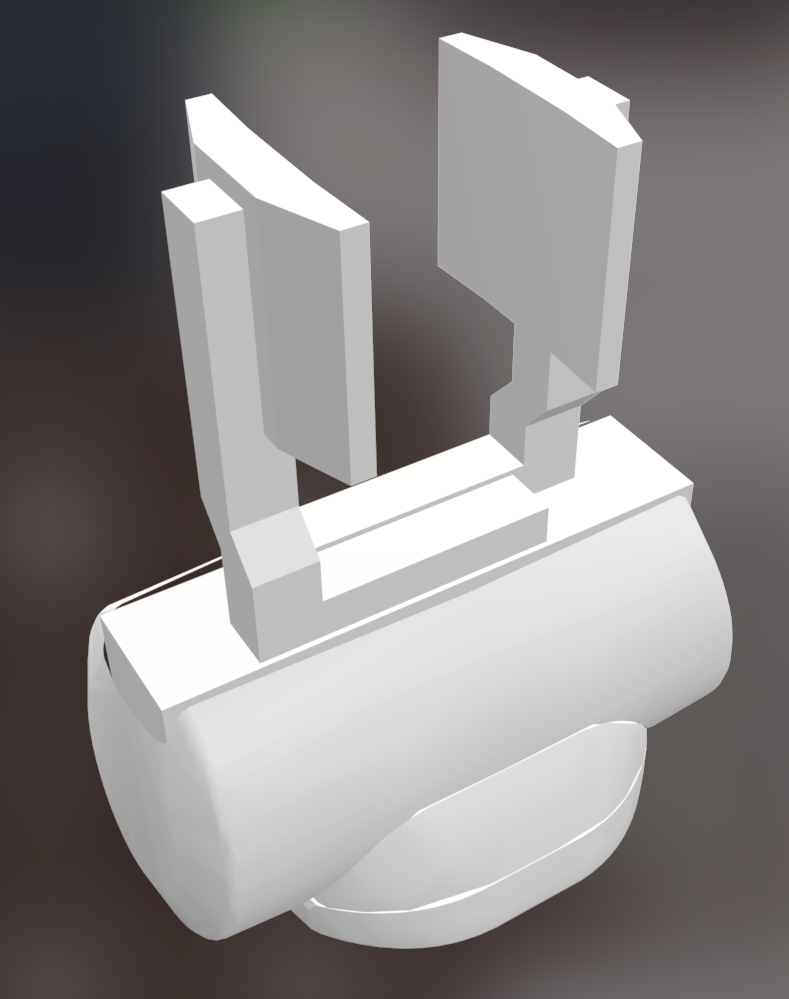
\includegraphics[width=.4\textwidth, trim={0 0 0 0}, clip]{img/gripper.png}
    \caption{Baxter gripper}
    \label{fig:coppelia_gripper}
\end{figure}
\end{frame}

\begin{frame}
\frametitle{Scene}
\framesubtitle{Robot control}
\begin{columns}[T]
\begin{column}{.48\textwidth}
\begin{itemize}
    \item The robot is entirely controlled by a custom user interface.
    \item The user can select the slot and the shelf of the cartridge to be loaded.
    \item The user can eject the currently loaded cartridge, which will be placed at its original slot.
\end{itemize}
\end{column}
\begin{column}{.48\textwidth}
\begin{figure}
    \centering
    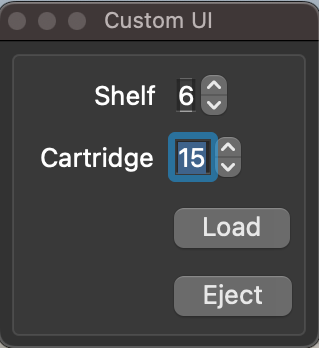
\includegraphics[scale=.7]{img/interface.png}
\end{figure}
\end{column}
\end{columns}
\end{frame}

\begin{frame}
\frametitle{Scene}
\framesubtitle{Robot control}
\begin{columns}[T]
\begin{column}{.48\textwidth}
\begin{itemize}
    \item If a tape is already loaded into the drive, the user can't load another tape.
    \item If a job is already in progress, the user can't request another operation.
    \item If a cartridge is not available at the required location, the operation is aborted.
\end{itemize}
\end{column}
\begin{column}{.48\textwidth}
\begin{figure}
    \centering
    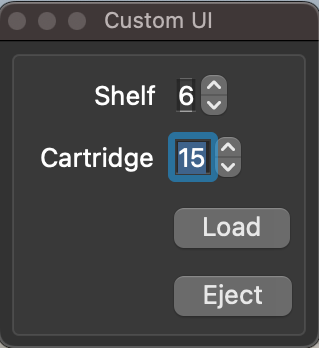
\includegraphics[scale=.7]{img/interface.png}
\end{figure}
\end{column}
\end{columns}
\end{frame}

\begin{frame}
\frametitle{Finite State Machine}
\framesubtitle{}
\begin{itemize}
    \item The robot control algorithm is driven by a finite state machine.
    \item The FSM is organized in four macro blocks, reflecting the four main tasks the robot has to carry out.
\end{itemize}
\end{frame}

\begin{frame}
\frametitle{Finite State Machine}
\framesubtitle{}
\begin{figure}
    \centering
    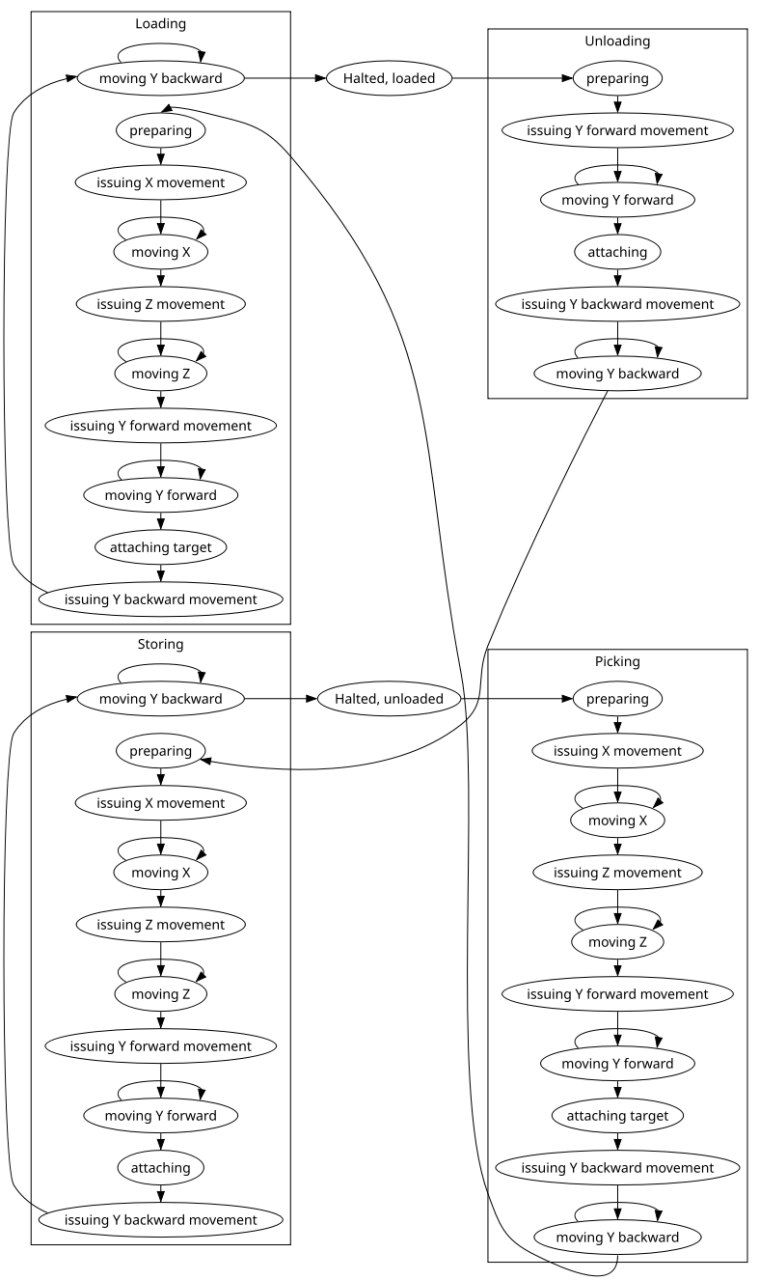
\includegraphics[trim={0 0 0 0}, clip, scale=.21]{img/fsm.jpg}
    \label{fig:state_machine}
\end{figure}
\end{frame}

\begin{frame}
\frametitle{Finite State Machine}
\framesubtitle{1/2}
\begin{itemize}
    \item \textbf{Picking}
    \begin{itemize}
        \item This sequence of actions is performed when the user asks for a cartridge to be loaded into the tape drive.
        \item The robot moves from its current position and aligns its end effector to the required cartridge, picking it from the shelf.
    \end{itemize}
    \item \textbf{Loading}
        \begin{itemize}
            \item This sequence of actions is performed after the picking stage.
            \item The robot aligns its end effector to the tape drive, loading the required cartridge.
        \end{itemize}
\end{itemize}
\end{frame}

\begin{frame}
\frametitle{Finite State Machine}
\framesubtitle{2/2}
\begin{itemize}
    \item \textbf{Unloading}
    \begin{itemize}
        \item This sequence of actions is performed when the user asks for the currently loaded cartridge in the tape drive to be ejected.
        \item The robot, whose end effector is already aligned to the tape drive, takes the cartridge from the drive.
    \end{itemize}
    \item \textbf{Storing}
    \begin{itemize}
        \item This sequence of actions is performed after the unloading stage.
        \item The end effector is aligned to the correct slot of the rack and the robot places the cartridge at its original location.
    \end{itemize}
\end{itemize}
\end{frame}

\begin{frame}
\[
position(shelf, slot) = 
\begin{bmatrix}
base_x + slot \times delta_x\\
offset_y \\
base_z + shelf \times delta_z
\end{bmatrix}
\]
\[
\begin{aligned}
base_x   &= 0.42 \, m\\
delta_x  &= distance + width\\
base_z   &= 0 \, m\\
delta_z  &= 0.15 \, m\\
distance &= 0.05 \, m\\
width    &= 0.02155 \, m\\
\end{aligned}
\]
\end{frame}

\begin{frame}[noframenumbering]{References}
\begin{thebibliography}{}
\bibitem{1}\href{https://www.youtube.com/watch?v=PwGY8PxQOXY&list=PLjzuoBhdtaXOoqkJUqhYQletLLnJP8vjZ}{A Complete CoppeliaSim Tutorial (V-REP), Leopoldo Armesto (Universitat Politècnica de València)}
\bibitem{2}\href{https://coppeliarobotics.com/helpFiles/index.html}{Coppelia user manual}

\end{thebibliography}
\end{frame}

\end{document}